\latex{\section*{Overview}\addcontentsline{toc}{subsection}{Overview}}
\latex{\label {sec:overview}}

\begin {htmlonly}
This package contains classes to produce charts used in the Java software developed in the {\em simulation laboratory\/}
of the DIRO, at the Universit\'e de Montr\'eal.
\end {htmlonly}

This package provides tools for easy
construction, visualization, and customization
of XY plots, histograms, and empirical styled charts
from a Java program.
It uses and extends the free and ``open source''
JFreeChart tool to manage the
charts. JFreeChart is
distributed under the terms of the GNU Lesser General Public License
(LGPL), and can be found at \url{http://www.jfree.org/jfreechart/}.

This package also provides facilities
to export charts to PGF/TikZ source code, which can be included into
\LaTeX\ documents. TikZ is a free \LaTeX{}
package to produce pictures such as plots, and can be downloaded from
\url{http://sourceforge.net/projects/pgf}.

The user does not need to be familiar with the JFreeChart package
or the TikZ syntax to
use these tools, except if customization is required.
For this, one may see the API specification of JFreeChart, and
the reference manual of TikZ.

The two basic abstract classes of package \texttt{charts} are
\externalclass{umontreal.iro.lecuyer.charts}{XYChart} and
\externalclass{umontreal.iro.lecuyer.charts}{CategoryChart}. All other
charts inherit from one of these two. Charts are managed by
the mother class which contains the data tables in a
\texttt{*SeriesCollection} object, and the
information about $x$-axis and $y$-axis in
\externalclass{umontreal.iro.lecuyer.charts}{Axis} instances.
All these objects encapsulate JFreeChart instances along with some
additional TikZ-specific attributes.
The method
\externalmethod{umontreal.iro.lecuyer.charts}{XYChart}{view}{}
displays charts on screen while the method
\texttt{toLatex} formats and returns a
\externalclass{java.lang}{String}{} which contains the TikZ source
code that can be written to a \LaTeX\ file.

Several chart styles are available and each one is represented by a
 subclass of \externalclass{umontreal.iro.lecuyer.charts}{XYChart} or of
\externalclass{umontreal.iro.lecuyer.charts}{CategoryChart}.
The \externalclass{umontreal.iro.lecuyer.charts}{XYLineChart} uses
\externalclass{umontreal.iro.lecuyer.charts}{XYListSeriesCollection}
to plot curves and lines, the
\externalclass{umontreal.iro.lecuyer.charts}{HistogramSeries\-Collection}
class is used by
\externalclass{umontreal.iro.lecuyer.charts}{HistogramChart} to plot
histograms, and the
\externalclass{umontreal.iro.lecuyer.charts}{EmpiricalSeries\-Collection} is used by
\externalclass{umontreal.iro.lecuyer.charts}{EmpiricalChart} to plot empirical style charts. It is possible to draw a scatter plot or a box plot using
\externalclass{umontreal.iro.lecuyer.charts}{ScatterChart} or
\externalclass{umontreal.iro.lecuyer.charts}{BoxChart} respectively.
These concrete subclasses have similar APIs, but they are specialized for
different kinds of charts.

These charts can be customized using
\texttt{*SeriesCollection} subclasses and
\externalclass{umontreal.iro.lecuyer.charts}{Axis}.
First, one can use methods in
the \externalclass{umontreal.iro.lecuyer.charts}{XYChart} class for
setting the range values and a background grid.
One can also use the method
\texttt{getSeriesCollection()} for subclasses of charts to obtain
the dataset of the chart, which is represented by a
\texttt{*SeriesCollection} object.
This dataset can be customized in the following ways by calling
methods
on the series collection:
selecting color, changing
plot style (straight lines, curves, marks only, \ldots), putting marks
on points, setting a label and selecting the dash pattern (solid,
dotted, dashed, \ldots). The available properties depend on the type
of chart.
Moreover, objects representing the axes can be retrieved with
\externalmethod{umontreal.iro.lecuyer.charts}{XYChart}{getXAxis}{}
for the
$x$-axis, and
\externalmethod{umontreal.iro.lecuyer.charts}{XYChart}{getYAxis}{}
for  the $y$-axis.
By using methods in \externalclass{umontreal.iro.lecuyer.charts}{Axis},
many customizations are possible: setting a label to the axis,
setting ticks labels and values (auto ticks, periodical ticks or
manually defined ticks) and changing the twin axis position on the
current axis to select where axes must appear.
These settings are independent for each axis.

Each chart object from SSJ encapsulates a JFreeChart object: a
\externalclass{umontreal.iro.lecuyer.charts}{XYChart} instance contains a
\texttt{JFreeChart} instance from JFreeChart API, a
\texttt{*SeriesCollection} contains a
\texttt{XYDataset} and a \texttt{XYItem\-Renderer}, and finally an
\externalclass{umontreal.iro.lecuyer.charts}{Axis} contains a
\texttt{NumberAxis}. So any parameter proposed by
JFreeChart  is reachable through
getter methods.  However,
changing the JFreeChart parameters directly may have no impact
on the produced TikZ source code.

The two special classes
\externalclass{umontreal.iro.lecuyer.charts}{ContinuousDistChart} and
\externalclass{umontreal.iro.lecuyer.charts}{DiscreteDistIntChart}
can be used to plot probability densities, mass functions,
and cumulative probabilities for continuous or discrete distributions,
which are implemented in package
\externalclass{umontreal.iro.lecuyer}{probdist} of SSJ.


The package \texttt{charts} provides additional tools for formatting
 data plot, and creating charts with multiple datasets. The
\externalclass{umontreal.iro.lecuyer.charts}{PlotFormat} class
offers basic tools to import and export data from files.
Supported file formats are GNUPlot and standard CSV, which is widely
used and accepted by most mathematical softwares such as
MATLAB and Mathematica. Customizing file input and output format is also possible.
Finally \externalclass{umontreal.iro.lecuyer.charts}{MultipleDatasetChart}
 provides tools to plot with different styles on the same chart.

\latex{\section*{Examples}\addcontentsline{toc}{subsection}{Examples}}
\latex{\label {sec:examples}}

\begin{htmlonly}
For a series of examples, see the \textbf{pdf} documentation.
\end{htmlonly}

\begin{latexonly}

The following examples demonstrate how to build charts with this package.

\lstinputlisting[label=lst:normalchart,%
caption={A simple example of chart creation},%
lineskip=-2pt,%
emph={getPoints,main}
]{exam/NormalChart.java}

\begin{figure}
% PGF/TikZ picture from SSJ 
% XScale = 100.0,  YScale = 1000.0,  XShift = 0.0,  YShift = 0.0
% Therefore, thisFileXValue = (originalSeriesXValue+XShift)*XScale
%        and thisFileYValue = (originalSeriesYValue+YShift)*YScale

\begin{center}
\begin{tikzpicture}[x=0.015cm, y=0.018604651162790697cm]
\footnotesize
\draw [latex-latex] ([xshift=-3mm] -400.0,0) -- ([xshift=3mm] 400.0,0) node[right] {X};
\draw (0.0,0) -- +(0mm,1mm) -- +(0mm,-1mm) node[below right] {0};
\draw (100.0,0) -- +(0mm,1mm) -- +(0mm,-1mm) node[below] {1};
\draw (200.0,0) -- +(0mm,1mm) -- +(0mm,-1mm) node[below] {2};
\draw (300.0,0) -- +(0mm,1mm) -- +(0mm,-1mm) node[below] {3};
\draw (400.0,0) -- +(0mm,1mm) -- +(0mm,-1mm) node[below] {4};
\draw (-100.0,0) -- +(0mm,1mm) -- +(0mm,-1mm) node[below] {-1};
\draw (-200.0,0) -- +(0mm,1mm) -- +(0mm,-1mm) node[below] {-2};
\draw (-300.0,0) -- +(0mm,1mm) -- +(0mm,-1mm) node[below] {-3};
\draw (-400.0,0) -- +(0mm,1mm) -- +(0mm,-1mm) node[below] {-4};
\draw [latex-latex] ([yshift=-3mm] 0,-10.0) -- ([yshift=3mm] 0, 420.0) node[above] { };
\draw (0,0.0) -- +(1mm,0mm) -- +(-1mm,0mm) node[above left] {0};
\draw (0,50.0) -- +(1mm,0mm) -- +(-1mm,0mm) node[left] {0.05};
\draw (0,100.0) -- +(1mm,0mm) -- +(-1mm,0mm) node[left] {0.1};
\draw (0,150.00000000000003) -- +(1mm,0mm) -- +(-1mm,0mm) node[left] {0.15};
\draw (0,200.0) -- +(1mm,0mm) -- +(-1mm,0mm) node[left] {0.2};
\draw (0,250.0) -- +(1mm,0mm) -- +(-1mm,0mm) node[left] {0.25};
\draw (0,300.0) -- +(1mm,0mm) -- +(-1mm,0mm) node[left] {0.3};
\draw (0,350.0) -- +(1mm,0mm) -- +(-1mm,0mm) node[left] {0.35};
\draw (0,399.99999999999994) -- +(1mm,0mm) -- +(-1mm,0mm) node[left] {0.4};
\draw [smooth, color=red, mark= , style=solid] plot coordinates {%
(-350.00,0.8727) %   (-3.500000,  0.000873)
(-320.83,2.3213) %   (-3.208333,  0.002321)
(-291.67,5.6709) %   (-2.916667,  0.005671)
(-262.50,12.7242) %   (-2.625000,  0.012724)
(-233.33,26.2219) %   (-2.333333,  0.026222)
(-204.17,49.6310) %   (-2.041667,  0.049631)
(-175.00,86.2773) %   (-1.750000,  0.086277)
(-145.83,137.7511) %   (-1.458333,  0.137751)
(-116.67,201.9987) %   (-1.166667,  0.201999)
(-87.50,272.0550) %   (-0.875000,  0.272055)
(-58.33,336.5268) %   (-0.583333,  0.336527)
(-29.17,382.3292) %   (-0.291667,  0.382329)
(0.00,398.9423) %   (0.000000,  0.398942)
(29.17,382.3292) %   (0.291667,  0.382329)
(58.33,336.5268) %   (0.583333,  0.336527)
(87.50,272.0550) %   (0.875000,  0.272055)
(116.67,201.9987) %   (1.166667,  0.201999)
(145.83,137.7511) %   (1.458333,  0.137751)
(175.00,86.2773) %   (1.750000,  0.086277)
(204.17,49.6310) %   (2.041667,  0.049631)
(233.33,26.2219) %   (2.333333,  0.026222)
(262.50,12.7242) %   (2.625000,  0.012724)
(291.67,5.6709) %   (2.916667,  0.005671)
(320.83,2.3213) %   (3.208333,  0.002321)
(350.00,0.8727)} %   (3.500000,  0.000873)
 node[right] { };
\end{tikzpicture}
\end{center}

\caption{The density of the standard normal.\label{fig:normalchart-res}}
\end{figure}


The first program, displayed in Listing~\ref{lst:normalchart},
shows the simplest way to export charts from data tables.
First, a curve is defined with regularly spaced $x$-coordinates
in method \texttt{getPoints}; it represents the curve
 $y = e^{-x^2/2}/\sqrt{2\pi}$, the density of the standard normal probability
 distribution. Arrays \texttt{points[0]} contain
the $x$-coordinates and \texttt{points[1]} the $y$-coordinates
of the points.
Figure~\ref{fig:normalchart-res} presents the resulting chart if the produced
TikZ code is added to a \LaTeX\ document using the \texttt{tikz}
package, and compiled using \LaTeX or Pdf\LaTeX.



%%%%%%%%%%%%%%%%%%%%%%%%%%%%%%%%%%%%%%%%%%%%%%

A simpler way to plot a
 probability density or a distribution function is to use the class
\externalclass{umontreal.iro.lecuyer.charts}{ContinuousDistChart}, as shown
in Listing~\ref{lst:normaldist}  where however, the normal density will be plotted
directly on the screen.

\lstinputlisting[label=lst:normaldist,%
caption={The normal density},%
lineskip=-1pt,%
emph={main}
]{exam/ContDistPlot.java}



%%%%%%%%%%%%%%%%%%%%%%%%%%%%%%%%%%%%%%%%%%%%%%

The next example, displayed in Listing~\ref{lst:poissonchart}, plots the
probability mass function for a Poisson distribution with $\lambda= 50$
by simply creating an instance of
\externalclass{umontreal.iro.lecuyer.charts}{DiscreteDistIntChart}.
Figure~\ref{fig:poissonchart-res} presents the resulting chart obtained
from PdfLaTeX.

\begin{figure}

% PGF/TikZ picture from SSJ: probability: PoissonDist: lambda = 50.0
% XScale = 10.0,  YScale = 10000.0,  XShift = 27.0,  YShift = 0.0
% Therefore, thisFileXValue = (originalSeriesXValue+XShift)*XScale
%        and thisFileYValue = (originalSeriesYValue+YShift)*YScale

\begin{center}
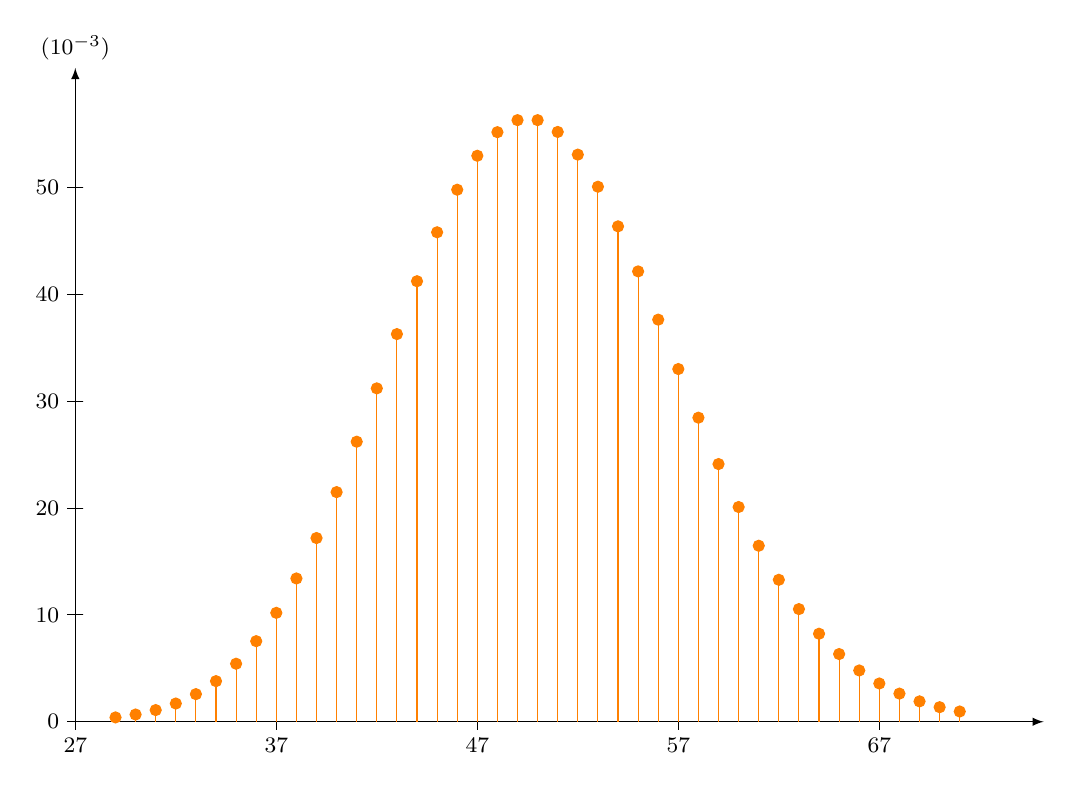
\begin{tikzpicture}[x=0.02553191489361702cm, y=0.013559322033898305cm]
\footnotesize
\draw [-latex] ([xshift=-0mm] 0.0,0) -- ([xshift=3mm] 470.0,0) node[right] {};
\draw (0.0,0) -- +(0mm,1mm) -- +(0mm,-1mm) node[below] {27};
\draw (100.0,0) -- +(0mm,1mm) -- +(0mm,-1mm) node[below] {37};
\draw (200.0,0) -- +(0mm,1mm) -- +(0mm,-1mm) node[below] {47};
\draw (300.0,0) -- +(0mm,1mm) -- +(0mm,-1mm) node[below] {57};
\draw (400.0,0) -- +(0mm,1mm) -- +(0mm,-1mm) node[below] {67};
\draw [-latex] ([yshift=-0mm] 0,0.0) -- ([yshift=3mm] 0, 590.0) node[above] { $(10^{-3})$};
\draw (0,0.0) -- +(1mm,0mm) -- +(-1mm,0mm) node[left] {0};
\draw (0,100.0) -- +(1mm,0mm) -- +(-1mm,0mm) node[left] {10};
\draw (0,200.0) -- +(1mm,0mm) -- +(-1mm,0mm) node[left] {20};
\draw (0,300.0) -- +(1mm,0mm) -- +(-1mm,0mm) node[left] {30};
\draw (0,400.0) -- +(1mm,0mm) -- +(-1mm,0mm) node[left] {40};
\draw (0,500.0) -- +(1mm,0mm) -- +(-1mm,0mm) node[left] {50};
\draw [ycomb, color=orange, mark=*, style=solid] plot coordinates {%
(20.00,4.0632) %   (29.000000,  0.000406)
(30.00,6.7720) %   (30.000000,  0.000677)
(40.00,10.9226) %   (31.000000,  0.001092)
(50.00,17.0665) %   (32.000000,  0.001707)
(60.00,25.8583) %   (33.000000,  0.002586)
(70.00,38.0269) %   (34.000000,  0.003803)
(80.00,54.3242) %   (35.000000,  0.005432)
(90.00,75.4503) %   (36.000000,  0.007545)
(100.00,101.9599) %   (37.000000,  0.010196)
(110.00,134.1577) %   (38.000000,  0.013416)
(120.00,171.9970) %   (39.000000,  0.017200)
(130.00,214.9963) %   (40.000000,  0.021500)
(140.00,262.1906) %   (41.000000,  0.026219)
(150.00,312.1317) %   (42.000000,  0.031213)
(160.00,362.9438) %   (43.000000,  0.036294)
(170.00,412.4362) %   (44.000000,  0.041244)
(180.00,458.2624) %   (45.000000,  0.045826)
(190.00,498.1113) %   (46.000000,  0.049811)
(200.00,529.9057) %   (47.000000,  0.052991)
(210.00,551.9851) %   (48.000000,  0.055199)
(220.00,563.2501) %   (49.000000,  0.056325)
(230.00,563.2501) %   (50.000000,  0.056325)
(240.00,552.2059) %   (51.000000,  0.055221)
(250.00,530.9673) %   (52.000000,  0.053097)
(260.00,500.9125) %   (53.000000,  0.050091)
(270.00,463.8079) %   (54.000000,  0.046381)
(280.00,421.6435) %   (55.000000,  0.042164)
(290.00,376.4674) %   (56.000000,  0.037647)
(300.00,330.2346) %   (57.000000,  0.033023)
(310.00,284.6850) %   (58.000000,  0.028468)
(320.00,241.2585) %   (59.000000,  0.024126)
(330.00,201.0487) %   (60.000000,  0.020105)
(340.00,164.7940) %   (61.000000,  0.016479)
(350.00,132.8984) %   (62.000000,  0.013290)
(360.00,105.4749) %   (63.000000,  0.010547)
(370.00,82.4023) %   (64.000000,  0.008240)
(380.00,63.3864) %   (65.000000,  0.006339)
(390.00,48.0200) %   (66.000000,  0.004802)
(400.00,35.8358) %   (67.000000,  0.003584)
(410.00,26.3499) %   (68.000000,  0.002635)
(420.00,19.0941) %   (69.000000,  0.001909)
(430.00,13.6386) %   (70.000000,  0.001364)
(440.00,9.6047)} %   (71.000000,  0.000960)
 node[right] { };
\end{tikzpicture}
\end{center}

\caption{The probabilities of the Poisson distribution with $\lambda= 50$.\label{fig:poissonchart-res}}
\end{figure}


\lstinputlisting[label=lst:poissonchart,%
caption={Probabilities of the Poisson distribution},%
lineskip=-1pt,%
emph={main}
]{exam/DistIntTest.java}


%%%%%%%%%%%%%%%%%%%%%%%%%%%%%%%%%%%%%%%%%%%%%%

The next program, displayed in Listing~\ref{lst:simplechart},
shows how to export several charts from data tables.
First, three curves are defined with regularly spaced $x$-coordinates
in methods \texttt{getPoints*}; they represent the curves $y = \sqrt x$,
$y = \cos(x)$ and $y = x+2$, respectively. Array \texttt{points[0]} contains
the $x$-coordinates and \texttt{points[1]} the $y$-coordinates
of the points.
Figure~\ref{fig:simplechart-res} presents the resulting chart if the produced
TikZ code is added to a \LaTeX\ document using the \texttt{tikz}
package, and compiled using \LaTeX  or PdfLaTeX.


\lstinputlisting[label=lst:simplechart,%
caption={Three curves on the same chart},%
lineskip=-1pt,%
emph={getPoints1,getPoints2,getPoints3,main}
]{exam/ChartTest1.java}


\begin{figure}
% PGF/TikZ picture from SSJ 
% XScale = 10.0,  YScale = 10.0,  XShift = -6.0,  YShift = -4.0
% Therefore, thisFileXValue = (originalSeriesXValue+XShift)*XScale
%        and thisFileYValue = (originalSeriesYValue+YShift)*YScale

\begin{center}
\begin{tikzpicture}[x=0.08cm, y=0.06666666666666667cm]
\footnotesize
\draw [-latex] ([xshift=-0mm] 0.0,0) -- ([xshift=3mm] 150.0,0) node[right] {X};
\draw (0.0,0) -- +(0mm,1mm) -- +(0mm,-1mm) node[below] {-6};
\draw (25.0,0) -- +(0mm,1mm) -- +(0mm,-1mm) node[below] {-3.5};
\draw (50.0,0) -- +(0mm,1mm) -- +(0mm,-1mm) node[below] {-1};
\draw (75.0,0) -- +(0mm,1mm) -- +(0mm,-1mm) node[below] {1.5};
\draw (100.0,0) -- +(0mm,1mm) -- +(0mm,-1mm) node[below] {4};
\draw (125.0,0) -- +(0mm,1mm) -- +(0mm,-1mm) node[below] {6.5};
\draw (150.0,0) -- +(0mm,1mm) -- +(0mm,-1mm) node[below] {9};
\draw [-latex] ([yshift=-0mm] 0,0.0) -- ([yshift=3mm] 0, 120.0) node[above] {Y};
\draw (0,0.0) -- +(1mm,0mm) -- +(-1mm,0mm) node[left] {-4};
\draw (0,25.0) -- +(1mm,0mm) -- +(-1mm,0mm) node[left] {-1.5};
\draw (0,50.0) -- +(1mm,0mm) -- +(-1mm,0mm) node[left] {1};
\draw (0,75.0) -- +(1mm,0mm) -- +(-1mm,0mm) node[left] {3.5};
\draw (0,100.0) -- +(1mm,0mm) -- +(-1mm,0mm) node[left] {6};
\draw [smooth, color=green, mark= , style=solid] plot coordinates {%
(10.00,10.0000) %   (-5.000000,  -3.000000)
(20.00,20.0000) %   (-4.000000,  -2.000000)
(30.00,30.0000) %   (-3.000000,  -1.000000)
(40.00,40.0000) %   (-2.000000,  0.000000)
(50.00,50.0000) %   (-1.000000,  1.000000)
(60.00,60.0000) %   (0.000000,  2.000000)
(70.00,70.0000) %   (1.000000,  3.000000)
(80.00,80.0000) %   (2.000000,  4.000000)
(90.00,90.0000) %   (3.000000,  5.000000)
(100.00,100.0000) %   (4.000000,  6.000000)
(110.00,110.0000)} %   (5.000000,  7.000000)
 node[right] { };
\draw [smooth, color=blue, mark= , style=solid] plot coordinates {%
(28.58,30.0000) %   (-3.141593,  -1.000000)
(31.73,30.4894) %   (-2.827433,  -0.951057)
(34.87,31.9098) %   (-2.513274,  -0.809017)
(38.01,34.1221) %   (-2.199115,  -0.587785)
(41.15,36.9098) %   (-1.884956,  -0.309017)
(44.29,40.0000) %   (-1.570796,  0.000000)
(47.43,43.0902) %   (-1.256637,  0.309017)
(50.58,45.8779) %   (-0.942478,  0.587785)
(53.72,48.0902) %   (-0.628319,  0.809017)
(56.86,49.5106) %   (-0.314159,  0.951057)
(60.00,50.0000) %   (0.000000,  1.000000)
(63.14,49.5106) %   (0.314159,  0.951057)
(66.28,48.0902) %   (0.628319,  0.809017)
(69.42,45.8779) %   (0.942478,  0.587785)
(72.57,43.0902) %   (1.256637,  0.309017)
(75.71,40.0000) %   (1.570796,  0.000000)
(78.85,36.9098) %   (1.884956,  -0.309017)
(81.99,34.1221) %   (2.199115,  -0.587785)
(85.13,31.9098) %   (2.513274,  -0.809017)
(88.27,30.4894) %   (2.827433,  -0.951057)
(91.42,30.0000)} %   (3.141593,  -1.000000)
 node[right] { };
\draw [smooth, color=red, mark= , style=solid] plot coordinates {%
(60.00,40.0000) %   (0.000000,  0.000000)
(60.40,42.0000) %   (0.040000,  0.200000)
(60.80,42.8284) %   (0.080000,  0.282843)
(61.20,43.4641) %   (0.120000,  0.346410)
(61.60,44.0000) %   (0.160000,  0.400000)
(62.00,44.4721) %   (0.200000,  0.447214)
(62.40,44.8990) %   (0.240000,  0.489898)
(62.80,45.2915) %   (0.280000,  0.529150)
(63.20,45.6569) %   (0.320000,  0.565685)
(63.60,46.0000) %   (0.360000,  0.600000)
(64.00,46.3246) %   (0.400000,  0.632456)
(64.40,46.6332) %   (0.440000,  0.663325)
(64.80,46.9282) %   (0.480000,  0.692820)
(65.20,47.2111) %   (0.520000,  0.721110)
(65.60,47.4833) %   (0.560000,  0.748331)
(66.00,47.7460) %   (0.600000,  0.774597)
(66.40,48.0000) %   (0.640000,  0.800000)
(66.80,48.2462) %   (0.680000,  0.824621)
(67.20,48.4853) %   (0.720000,  0.848528)
(67.60,48.7178) %   (0.760000,  0.871780)
(68.00,48.9443) %   (0.800000,  0.894427)
(68.40,49.1652) %   (0.840000,  0.916515)
(68.80,49.3808) %   (0.880000,  0.938083)
(69.20,49.5917) %   (0.920000,  0.959166)
(69.60,49.7980) %   (0.960000,  0.979796)
(70.00,50.0000) %   (1.000000,  1.000000)
(70.40,50.1980) %   (1.040000,  1.019804)
(70.80,50.3923) %   (1.080000,  1.039230)
(71.20,50.5830) %   (1.120000,  1.058301)
(71.60,50.7703) %   (1.160000,  1.077033)
(72.00,50.9545) %   (1.200000,  1.095445)
(72.40,51.1355) %   (1.240000,  1.113553)
(72.80,51.3137) %   (1.280000,  1.131371)
(73.20,51.4891) %   (1.320000,  1.148913)
(73.60,51.6619) %   (1.360000,  1.166190)
(74.00,51.8322) %   (1.400000,  1.183216)
(74.40,52.0000) %   (1.440000,  1.200000)
(74.80,52.1655) %   (1.480000,  1.216553)
(75.20,52.3288) %   (1.520000,  1.232883)
(75.60,52.4900) %   (1.560000,  1.249000)
(76.00,52.6491) %   (1.600000,  1.264911)
(76.40,52.8062) %   (1.640000,  1.280625)
(76.80,52.9615) %   (1.680000,  1.296148)
(77.20,53.1149) %   (1.720000,  1.311488)
(77.60,53.2665) %   (1.760000,  1.326650)
(78.00,53.4164) %   (1.800000,  1.341641)
(78.40,53.5647) %   (1.840000,  1.356466)
(78.80,53.7113) %   (1.880000,  1.371131)
(79.20,53.8564) %   (1.920000,  1.385641)
(79.60,54.0000) %   (1.960000,  1.400000)
(80.00,54.1421) %   (2.000000,  1.414214)
(80.40,54.2829) %   (2.040000,  1.428286)
(80.80,54.4222) %   (2.080000,  1.442221)
(81.20,54.5602) %   (2.120000,  1.456022)
(81.60,54.6969) %   (2.160000,  1.469694)
(82.00,54.8324) %   (2.200000,  1.483240)
(82.40,54.9666) %   (2.240000,  1.496663)
(82.80,55.0997) %   (2.280000,  1.509967)
(83.20,55.2315) %   (2.320000,  1.523155)
(83.60,55.3623) %   (2.360000,  1.536229)
(84.00,55.4919) %   (2.400000,  1.549193)
(84.40,55.6205) %   (2.440000,  1.562050)
(84.80,55.7480) %   (2.480000,  1.574802)
(85.20,55.8745) %   (2.520000,  1.587451)
(85.60,56.0000) %   (2.560000,  1.600000)
(86.00,56.1245) %   (2.600000,  1.612452)
(86.40,56.2481) %   (2.640000,  1.624808)
(86.80,56.3707) %   (2.680000,  1.637071)
(87.20,56.4924) %   (2.720000,  1.649242)
(87.60,56.6132) %   (2.760000,  1.661325)
(88.00,56.7332) %   (2.800000,  1.673320)
(88.40,56.8523) %   (2.840000,  1.685230)
(88.80,56.9706) %   (2.880000,  1.697056)
(89.20,57.0880) %   (2.920000,  1.708801)
(89.60,57.2047) %   (2.960000,  1.720465)
(90.00,57.3205) %   (3.000000,  1.732051)
(90.40,57.4356) %   (3.040000,  1.743560)
(90.80,57.5499) %   (3.080000,  1.754993)
(91.20,57.6635) %   (3.120000,  1.766352)
(91.60,57.7764) %   (3.160000,  1.777639)
(92.00,57.8885) %   (3.200000,  1.788854)
(92.40,58.0000) %   (3.240000,  1.800000)
(92.80,58.1108) %   (3.280000,  1.811077)
(93.20,58.2209) %   (3.320000,  1.822087)
(93.60,58.3303) %   (3.360000,  1.833030)
(94.00,58.4391) %   (3.400000,  1.843909)
(94.40,58.5472) %   (3.440000,  1.854724)
(94.80,58.6548) %   (3.480000,  1.865476)
(95.20,58.7617) %   (3.520000,  1.876166)
(95.60,58.8680) %   (3.560000,  1.886796)
(96.00,58.9737) %   (3.600000,  1.897367)
(96.40,59.0788) %   (3.640000,  1.907878)
(96.80,59.1833) %   (3.680000,  1.918333)
(97.20,59.2873) %   (3.720000,  1.928730)
(97.60,59.3907) %   (3.760000,  1.939072)
(98.00,59.4936) %   (3.800000,  1.949359)
(98.40,59.5959) %   (3.840000,  1.959592)
(98.80,59.6977) %   (3.880000,  1.969772)
(99.20,59.7990) %   (3.920000,  1.979899)
(99.60,59.8997) %   (3.960000,  1.989975)
(100.00,60.0000) %   (4.000000,  2.000000)
(100.40,60.0998) %   (4.040000,  2.009975)
(100.80,60.1990) %   (4.080000,  2.019901)
(101.20,60.2978) %   (4.120000,  2.029778)
(101.60,60.3961) %   (4.160000,  2.039608)
(102.00,60.4939) %   (4.200000,  2.049390)
(102.40,60.5913) %   (4.240000,  2.059126)
(102.80,60.6882) %   (4.280000,  2.068816)
(103.20,60.7846) %   (4.320000,  2.078461)
(103.60,60.8806) %   (4.360000,  2.088061)
(104.00,60.9762) %   (4.400000,  2.097618)
(104.40,61.0713) %   (4.440000,  2.107131)
(104.80,61.1660) %   (4.480000,  2.116601)
(105.20,61.2603) %   (4.520000,  2.126029)
(105.60,61.3542) %   (4.560000,  2.135416)
(106.00,61.4476) %   (4.600000,  2.144761)
(106.40,61.5407) %   (4.640000,  2.154066)
(106.80,61.6333) %   (4.680000,  2.163331)
(107.20,61.7256) %   (4.720000,  2.172556)
(107.60,61.8174) %   (4.760000,  2.181742)
(108.00,61.9089) %   (4.800000,  2.190890)
(108.40,62.0000) %   (4.840000,  2.200000)
(108.80,62.0907) %   (4.880000,  2.209072)
(109.20,62.1811) %   (4.920000,  2.218107)
(109.60,62.2711) %   (4.960000,  2.227106)
(110.00,62.3607) %   (5.000000,  2.236068)
(110.40,62.4499) %   (5.040000,  2.244994)
(110.80,62.5389) %   (5.080000,  2.253886)
(111.20,62.6274) %   (5.120000,  2.262742)
(111.60,62.7156) %   (5.160000,  2.271563)
(112.00,62.8035) %   (5.200000,  2.280351)
(112.40,62.8910) %   (5.240000,  2.289105)
(112.80,62.9783) %   (5.280000,  2.297825)
(113.20,63.0651) %   (5.320000,  2.306513)
(113.60,63.1517) %   (5.360000,  2.315167)
(114.00,63.2379) %   (5.400000,  2.323790)
(114.40,63.3238) %   (5.440000,  2.332381)
(114.80,63.4094) %   (5.480000,  2.340940)
(115.20,63.4947) %   (5.520000,  2.349468)
(115.60,63.5797) %   (5.560000,  2.357965)
(116.00,63.6643) %   (5.600000,  2.366432)
(116.40,63.7487) %   (5.640000,  2.374868)
(116.80,63.8328) %   (5.680000,  2.383275)
(117.20,63.9165) %   (5.720000,  2.391652)
(117.60,64.0000) %   (5.760000,  2.400000)
(118.00,64.0832) %   (5.800000,  2.408319)
(118.40,64.1661) %   (5.840000,  2.416609)
(118.80,64.2487) %   (5.880000,  2.424871)
(119.20,64.3311) %   (5.920000,  2.433105)
(119.60,64.4131) %   (5.960000,  2.441311)
(120.00,64.4949) %   (6.000000,  2.449490)
(120.40,64.5764) %   (6.040000,  2.457641)
(120.80,64.6577) %   (6.080000,  2.465766)
(121.20,64.7386) %   (6.120000,  2.473863)
(121.60,64.8193) %   (6.160000,  2.481935)
(122.00,64.8998) %   (6.200000,  2.489980)
(122.40,64.9800) %   (6.240000,  2.497999)
(122.80,65.0599) %   (6.280000,  2.505993)
(123.20,65.1396) %   (6.320000,  2.513961)
(123.60,65.2190) %   (6.360000,  2.521904)
(124.00,65.2982) %   (6.400000,  2.529822)
(124.40,65.3772) %   (6.440000,  2.537716)
(124.80,65.4558) %   (6.480000,  2.545584)
(125.20,65.5343) %   (6.520000,  2.553429)
(125.60,65.6125) %   (6.560000,  2.561250)
(126.00,65.6905) %   (6.600000,  2.569047)
(126.40,65.7682) %   (6.640000,  2.576820)
(126.80,65.8457) %   (6.680000,  2.584570)
(127.20,65.9230) %   (6.720000,  2.592296)
(127.60,66.0000) %   (6.760000,  2.600000)
(128.00,66.0768) %   (6.800000,  2.607681)
(128.40,66.1534) %   (6.840000,  2.615339)
(128.80,66.2298) %   (6.880000,  2.622975)
(129.20,66.3059) %   (6.920000,  2.630589)
(129.60,66.3818) %   (6.960000,  2.638181)
(130.00,66.4575) %   (7.000000,  2.645751)
(130.40,66.5330) %   (7.040000,  2.653300)
(130.80,66.6083) %   (7.080000,  2.660827)
(131.20,66.6833) %   (7.120000,  2.668333)
(131.60,66.7582) %   (7.160000,  2.675818)
(132.00,66.8328) %   (7.200000,  2.683282)
(132.40,66.9072) %   (7.240000,  2.690725)
(132.80,66.9815) %   (7.280000,  2.698148)
(133.20,67.0555) %   (7.320000,  2.705550)
(133.60,67.1293) %   (7.360000,  2.712932)
(134.00,67.2029) %   (7.400000,  2.720294)
(134.40,67.2764) %   (7.440000,  2.727636)
(134.80,67.3496) %   (7.480000,  2.734959)
(135.20,67.4226) %   (7.520000,  2.742262)
(135.60,67.4955) %   (7.560000,  2.749545)
(136.00,67.5681) %   (7.600000,  2.756810)
(136.40,67.6405) %   (7.640000,  2.764055)
(136.80,67.7128) %   (7.680000,  2.771281)
(137.20,67.7849) %   (7.720000,  2.778489)
(137.60,67.8568) %   (7.760000,  2.785678)
(138.00,67.9285) %   (7.800000,  2.792848)
(138.40,68.0000) %   (7.840000,  2.800000)
(138.80,68.0713) %   (7.880000,  2.807134)
(139.20,68.1425) %   (7.920000,  2.814249)
(139.60,68.2135)} %   (7.960000,  2.821347)
 node[right] { };
\end{tikzpicture}
\end{center}

\caption{Results for three curves on the same chart.\label{fig:simplechart-res}}
\end{figure}

%%%%%%%%%%%%%%%%%%%%%%%%%%%%%%%%%%%%%%%%%%%%%%



The next example, given in Listing~\ref{lst:customchart},
 shows how to customize a chart. First, three curves are defined as
in example~\ref{lst:simplechart} above and the chart is created. Then the
axes are customized by adding labels at chosen values on the $x$-axis.
On the $y$-axis, successive labels are set regularly at points 1 unit apart.
Then the data plot itself is customized. A new color is created in the RGB
model for the first curve which also receives a label name and a dash plot style.
Similarly, the other two curves receive their label name, plot style
 and color. Note that the third curve is drawn in the ORANGE color predefined
 in the AWT package of the standard Java toolkit.
Finally, the charts are exported to a file in \LaTeX{}
format. If the file is compiled with \LaTeX{} or PdfLaTeX, the
resulting chart will appear as  displayed in Figure~\ref{fig:customchart-res}.


\lstinputlisting[label=lst:customchart,%
caption={Code for creating and customizing a chart},%
lineskip=-1pt,%
emph={getPoints1,getPoints2,getPoints3,main}
]{exam/ChartTest2.java}


\begin{figure}
% PGF/TikZ picture from SSJ 
% XScale = 10.0,  YScale = 10.0,  XShift = -6.0,  YShift = -4.0
% Therefore, thisFileXValue = (originalSeriesXValue+XShift)*XScale
%        and thisFileYValue = (originalSeriesYValue+YShift)*YScale

\begin{center}
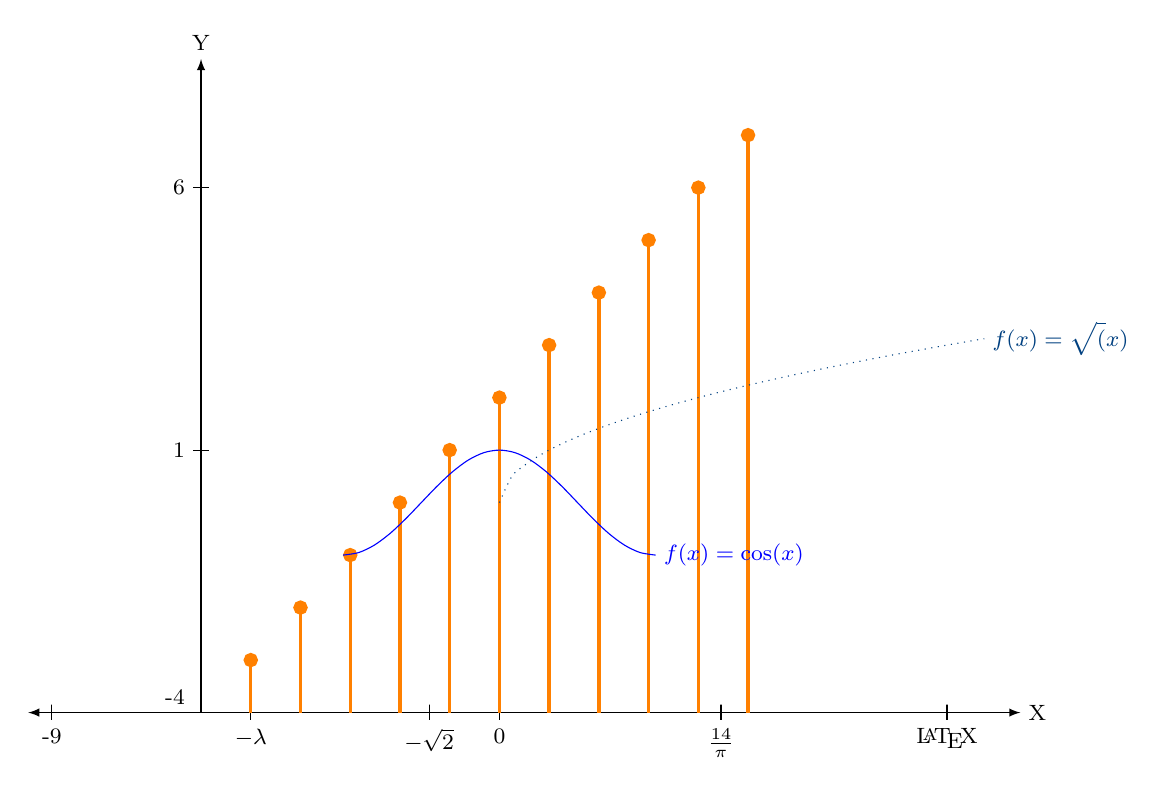
\begin{tikzpicture}[x=0.06315789473684211cm, y=0.06666666666666667cm]
\footnotesize
\draw [latex-latex] ([xshift=-3mm] -30.0,0) -- ([xshift=3mm] 160.0,0) node[right] {X};
\draw (-30.0,0) -- +(0mm,1mm) -- +(0mm,-1mm) node[below] {-9};
\draw (10.0,0) -- +(0mm,1mm) -- +(0mm,-1mm) node[below] {$-\lambda$};
\draw (45.85786437626905,0) -- +(0mm,1mm) -- +(0mm,-1mm) node[below] {$-\sqrt{2}$};
\draw (60.0,0) -- +(0mm,1mm) -- +(0mm,-1mm) node[below] {0};
\draw (104.5633840657307,0) -- +(0mm,1mm) -- +(0mm,-1mm) node[below] {$\frac{14}{\pi}$};
\draw (150.0,0) -- +(0mm,1mm) -- +(0mm,-1mm) node[below] {\LaTeX};
\draw [-latex] ([yshift=-0mm] 0,0.0) -- ([yshift=3mm] 0, 120.0) node[above] {Y};
\draw (0,0.0) -- +(1mm,0mm) -- +(-1mm,0mm) node[above left] {-4};
\draw (0,50.0) -- +(1mm,0mm) -- +(-1mm,0mm) node[left] {1};
\draw (0,100.0) -- +(1mm,0mm) -- +(-1mm,0mm) node[left] {6};
\draw [ycomb,very thick, color=orange, mark=*, style=solid] plot coordinates {%
(10.00,10.0000) %   (-5.000000,  -3.000000)
(20.00,20.0000) %   (-4.000000,  -2.000000)
(30.00,30.0000) %   (-3.000000,  -1.000000)
(40.00,40.0000) %   (-2.000000,  0.000000)
(50.00,50.0000) %   (-1.000000,  1.000000)
(60.00,60.0000) %   (0.000000,  2.000000)
(70.00,70.0000) %   (1.000000,  3.000000)
(80.00,80.0000) %   (2.000000,  4.000000)
(90.00,90.0000) %   (3.000000,  5.000000)
(100.00,100.0000) %   (4.000000,  6.000000)
(110.00,110.0000)} %   (5.000000,  7.000000)
 node[right] { };
\draw [smooth, color=blue, mark=, style=solid] plot coordinates {%
(28.58,30.0000) %   (-3.141593,  -1.000000)
(31.73,30.4894) %   (-2.827433,  -0.951057)
(34.87,31.9098) %   (-2.513274,  -0.809017)
(38.01,34.1221) %   (-2.199115,  -0.587785)
(41.15,36.9098) %   (-1.884956,  -0.309017)
(44.29,40.0000) %   (-1.570796,  0.000000)
(47.43,43.0902) %   (-1.256637,  0.309017)
(50.58,45.8779) %   (-0.942478,  0.587785)
(53.72,48.0902) %   (-0.628319,  0.809017)
(56.86,49.5106) %   (-0.314159,  0.951057)
(60.00,50.0000) %   (0.000000,  1.000000)
(63.14,49.5106) %   (0.314159,  0.951057)
(66.28,48.0902) %   (0.628319,  0.809017)
(69.42,45.8779) %   (0.942478,  0.587785)
(72.57,43.0902) %   (1.256637,  0.309017)
(75.71,40.0000) %   (1.570796,  0.000000)
(78.85,36.9098) %   (1.884956,  -0.309017)
(81.99,34.1221) %   (2.199115,  -0.587785)
(85.13,31.9098) %   (2.513274,  -0.809017)
(88.27,30.4894) %   (2.827433,  -0.951057)
(91.42,30.0000)} %   (3.141593,  -1.000000)
 node[right] {$f(x) = \cos(x)$};
\definecolor{color0}{rgb}{0.00, 0.25, 0.50}
\draw [smooth, color=color0, mark=, style=dotted] plot coordinates {%
(60.00,40.0000) %   (0.000000,  0.000000)
(62.50,45.0000) %   (0.250000,  0.500000)
(65.00,47.0711) %   (0.500000,  0.707107)
(67.50,48.6603) %   (0.750000,  0.866025)
(70.00,50.0000) %   (1.000000,  1.000000)
(72.50,51.1803) %   (1.250000,  1.118034)
(75.00,52.2474) %   (1.500000,  1.224745)
(77.50,53.2288) %   (1.750000,  1.322876)
(80.00,54.1421) %   (2.000000,  1.414214)
(82.50,55.0000) %   (2.250000,  1.500000)
(85.00,55.8114) %   (2.500000,  1.581139)
(87.50,56.5831) %   (2.750000,  1.658312)
(90.00,57.3205) %   (3.000000,  1.732051)
(92.50,58.0278) %   (3.250000,  1.802776)
(95.00,58.7083) %   (3.500000,  1.870829)
(97.50,59.3649) %   (3.750000,  1.936492)
(100.00,60.0000) %   (4.000000,  2.000000)
(102.50,60.6155) %   (4.250000,  2.061553)
(105.00,61.2132) %   (4.500000,  2.121320)
(107.50,61.7945) %   (4.750000,  2.179449)
(110.00,62.3607) %   (5.000000,  2.236068)
(112.50,62.9129) %   (5.250000,  2.291288)
(115.00,63.4521) %   (5.500000,  2.345208)
(117.50,63.9792) %   (5.750000,  2.397916)
(120.00,64.4949) %   (6.000000,  2.449490)
(122.50,65.0000) %   (6.250000,  2.500000)
(125.00,65.4951) %   (6.500000,  2.549510)
(127.50,65.9808) %   (6.750000,  2.598076)
(130.00,66.4575) %   (7.000000,  2.645751)
(132.50,66.9258) %   (7.250000,  2.692582)
(135.00,67.3861) %   (7.500000,  2.738613)
(137.50,67.8388) %   (7.750000,  2.783882)
(140.00,68.2843) %   (8.000000,  2.828427)
(142.50,68.7228) %   (8.250000,  2.872281)
(145.00,69.1548) %   (8.500000,  2.915476)
(147.50,69.5804) %   (8.750000,  2.958040)
(150.00,70.0000) %   (9.000000,  3.000000)
(152.50,70.4138) %   (9.250000,  3.041381)
(155.00,70.8221) %   (9.500000,  3.082207)
(157.50,71.2250)} %   (9.750000,  3.122499)
 node[right] {$f(x) = \sqrt(x)$};
\end{tikzpicture}
\end{center}


\caption{A customized chart.\label{fig:customchart-res}}
\end{figure}

%%%%%%%%%%%%%%%%%%%%%%%%%%%%%%%%%%%%%%%%%%%%%%


The next example, given in Listing~\ref{lst:empiricalchart}, shows how to
plot and customize empirical distributions. First, two empirical distributions
are defined from a sample of points obtained from a uniform
generator and a Beta$(3, 1)$ generator, both on the interval
$[0, 1]$. Then an empirical chart is
created to plot these two distributions. The first distribution is plotted
in MAGENTA color with filled square marks from TikZ. The second distribution
uses default color and plot marks. A background grid is also added with cells
of size $0.1\times 0.1$. Finally, the charts are exported to a file in \LaTeX{} format. Figure~\ref{fig:empiricalchart-res} shows the
resulting chart.


\lstinputlisting[label=lst:empiricalchart,%
caption={Creating and customizing empirical distribution charts},%
lineskip=-1pt,%
emph={getPoints1,getPoints2,main}
]{exam/EmpiricalChartTest.java}


\begin{figure}

% PGF/TikZ picture from SSJ 
% XScale = 1000.0,  YScale = 100.0,  XShift = 0.0,  YShift = 0.0
% Therefore, thisFileXValue = (originalSeriesXValue+XShift)*XScale
%        and thisFileYValue = (originalSeriesYValue+YShift)*YScale

\begin{center}
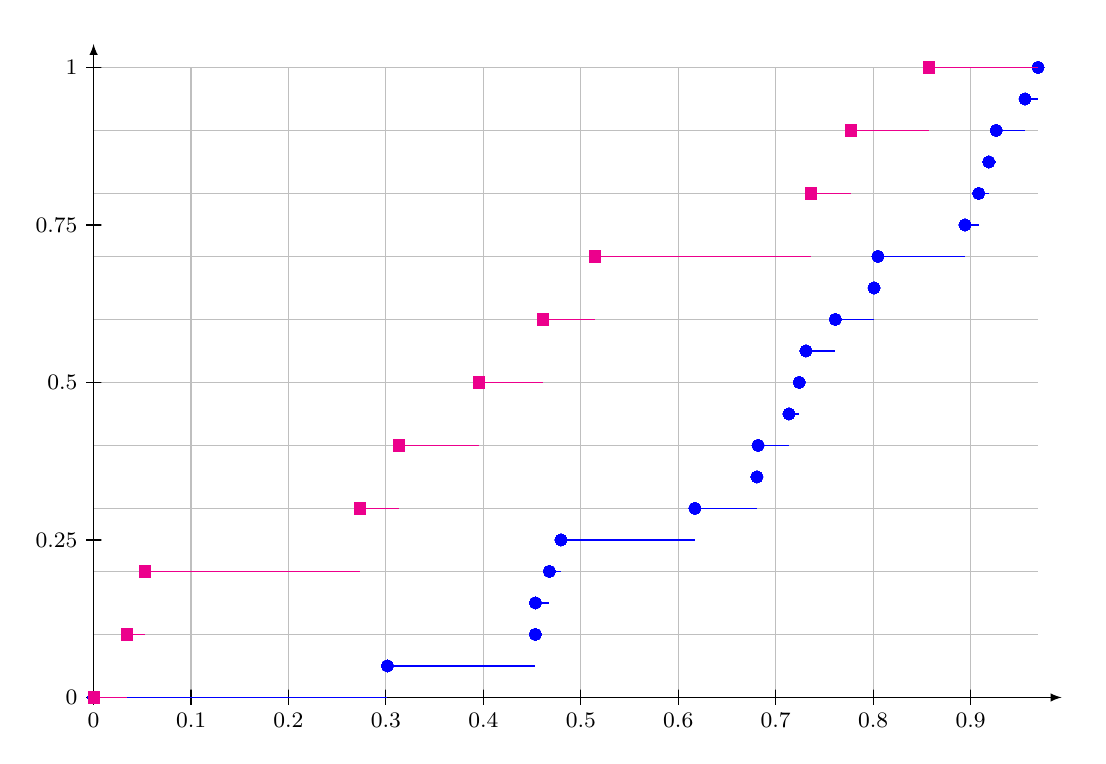
\begin{tikzpicture}[x=0.012380800583714944cm, y=0.08cm]
\footnotesize
\draw[color=lightgray] (0.0, 0.0) grid[xstep = 100.0, ystep=10.0] (969.2426526749952, 100.0);
\draw [-latex] ([xshift=-0mm] 0.0,0) -- ([xshift=3mm] 969.2426526749952,0) node[right] { };
\draw (0.0,0) -- +(0mm,1mm) -- +(0mm,-1mm) node[below] {0};
\draw (100.0,0) -- +(0mm,1mm) -- +(0mm,-1mm) node[below] {0.1};
\draw (200.0,0) -- +(0mm,1mm) -- +(0mm,-1mm) node[below] {0.2};
\draw (300.00000000000006,0) -- +(0mm,1mm) -- +(0mm,-1mm) node[below] {0.3};
\draw (400.0,0) -- +(0mm,1mm) -- +(0mm,-1mm) node[below] {0.4};
\draw (500.0,0) -- +(0mm,1mm) -- +(0mm,-1mm) node[below] {0.5};
\draw (600.0,0) -- +(0mm,1mm) -- +(0mm,-1mm) node[below] {0.6};
\draw (700.0,0) -- +(0mm,1mm) -- +(0mm,-1mm) node[below] {0.7};
\draw (799.9999999999999,0) -- +(0mm,1mm) -- +(0mm,-1mm) node[below] {0.8};
\draw (899.9999999999999,0) -- +(0mm,1mm) -- +(0mm,-1mm) node[below] {0.9};
\draw [-latex] ([yshift=-0mm] 0,0.0) -- ([yshift=3mm] 0, 100.0) node[above] { };
\draw (0,0.0) -- +(1mm,0mm) -- +(-1mm,0mm) node[left] {0};
\draw (0,25.0) -- +(1mm,0mm) -- +(-1mm,0mm) node[left] {0.25};
\draw (0,50.0) -- +(1mm,0mm) -- +(-1mm,0mm) node[left] {0.5};
\draw (0,75.0) -- +(1mm,0mm) -- +(-1mm,0mm) node[left] {0.75};
\draw (0,100.0) -- +(1mm,0mm) -- +(-1mm,0mm) node[left] {1};
\draw [color=blue] plot[mark=*] (0.0000, 0.0000) --plot[style=solid] (301.5304, 0.0000); %
\draw [color=blue] plot[mark=*] (301.5304, 5.0000) --plot[style=solid] (453.3903, 5.0000); %
\draw [color=blue] plot[mark=*] (453.3903, 10.0000) --plot[style=solid] (453.4337, 10.0000); %
\draw [color=blue] plot[mark=*] (453.4337, 15.0000) --plot[style=solid] (467.7741, 15.0000); %
\draw [color=blue] plot[mark=*] (467.7741, 20.0000) --plot[style=solid] (479.6471, 20.0000); %
\draw [color=blue] plot[mark=*] (479.6471, 25.0000) --plot[style=solid] (617.1170, 25.0000); %
\draw [color=blue] plot[mark=*] (617.1170, 30.0000) --plot[style=solid] (680.7208, 30.0000); %
\draw [color=blue] plot[mark=*] (680.7208, 35.0000) --plot[style=solid] (681.9469, 35.0000); %
\draw [color=blue] plot[mark=*] (681.9469, 40.0000) --plot[style=solid] (713.6196, 40.0000); %
\draw [color=blue] plot[mark=*] (713.6196, 45.0000) --plot[style=solid] (724.2162, 45.0000); %
\draw [color=blue] plot[mark=*] (724.2162, 50.0000) --plot[style=solid] (731.0242, 50.0000); %
\draw [color=blue] plot[mark=*] (731.0242, 55.0000) --plot[style=solid] (761.2374, 55.0000); %
\draw [color=blue] plot[mark=*] (761.2374, 60.0000) --plot[style=solid] (800.9418, 60.0000); %
\draw [color=blue] plot[mark=*] (800.9418, 65.0000) --plot[style=solid] (804.9549, 65.0000); %
\draw [color=blue] plot[mark=*] (804.9549, 70.0000) --plot[style=solid] (894.2900, 70.0000); %
\draw [color=blue] plot[mark=*] (894.2900, 75.0000) --plot[style=solid] (908.3347, 75.0000); %
\draw [color=blue] plot[mark=*] (908.3347, 80.0000) --plot[style=solid] (918.6914, 80.0000); %
\draw [color=blue] plot[mark=*] (918.6914, 85.0000) --plot[style=solid] (926.3442, 85.0000); %
\draw [color=blue] plot[mark=*] (926.3442, 90.0000) --plot[style=solid] (955.9302, 90.0000); %
\draw [color=blue] plot[mark=*] (955.9302, 95.0000) --plot[style=solid] (969.2427, 95.0000); %
\draw [color=blue] plot[mark=*] (969.2427, 100.0000) --plot[style=solid] (969.2427, 100.0000); %
\draw [color=magenta] plot[mark=square*] (0.0000, 0.0000) --plot[style=solid] (34.2733, 0.0000); %
\draw [color=magenta] plot[mark=square*] (34.2733, 10.0000) --plot[style=solid] (52.9135, 10.0000); %
\draw [color=magenta] plot[mark=square*] (52.9135, 20.0000) --plot[style=solid] (273.4031, 20.0000); %
\draw [color=magenta] plot[mark=square*] (273.4031, 30.0000) --plot[style=solid] (313.6786, 30.0000); %
\draw [color=magenta] plot[mark=square*] (313.6786, 40.0000) --plot[style=solid] (395.3887, 40.0000); %
\draw [color=magenta] plot[mark=square*] (395.3887, 50.0000) --plot[style=solid] (460.9833, 50.0000); %
\draw [color=magenta] plot[mark=square*] (460.9833, 60.0000) --plot[style=solid] (514.2070, 60.0000); %
\draw [color=magenta] plot[mark=square*] (514.2070, 70.0000) --plot[style=solid] (736.6297, 70.0000); %
\draw [color=magenta] plot[mark=square*] (736.6297, 80.0000) --plot[style=solid] (777.2346, 80.0000); %
\draw [color=magenta] plot[mark=square*] (777.2346, 90.0000) --plot[style=solid] (857.6070, 90.0000); %
\draw [color=magenta] plot[mark=square*] (857.6070, 100.0000) --plot[style=solid] (969.2427, 100.0000); %
\end{tikzpicture}
\end{center}


\caption{A customized empirical distribution chart\label {fig:empiricalchart-res}}
\end{figure}

% \clearpage
%%%%%%%%%%%%%%%%%%%%%%%%%%%%%%%%%%%%%%%%%%%%%%

The next example, given in Listing~\ref{lst:histo1}, shows how to plot
a simple histogram. First,  data is generated from a standard normal.
 Then the plot is customized: 80 bins are selected, and the range of the
  plot is set manually with \texttt{bounds}; the interval is $[-4, 4]$ for
   the $x$-coordinates, and $[0, 5000]$ for the $y$-coordinates.
 Finally, the histogram chart is viewed on the screen, then exported to
  file \texttt{HistogramTest1.tex} in
\LaTeX{} format.  Figure~\ref{fig:histo1-res} displays the resulting chart.


\lstinputlisting[label=lst:histo1,%
caption={Source code creating a simple histogram},%
lineskip=-1pt,%
emph={getData,main}
]{exam/HistogramTest1.java}


\begin{figure}
% PGF/TikZ picture from SSJ: Standard Normal
% XScale = 100.0,  YScale = 0.1,  XShift = -4.0,  YShift = 0.0
% Therefore, thisFileXValue = (originalSeriesXValue+XShift)*XScale
%        and thisFileYValue = (originalSeriesYValue+YShift)*YScale

\begin{center}
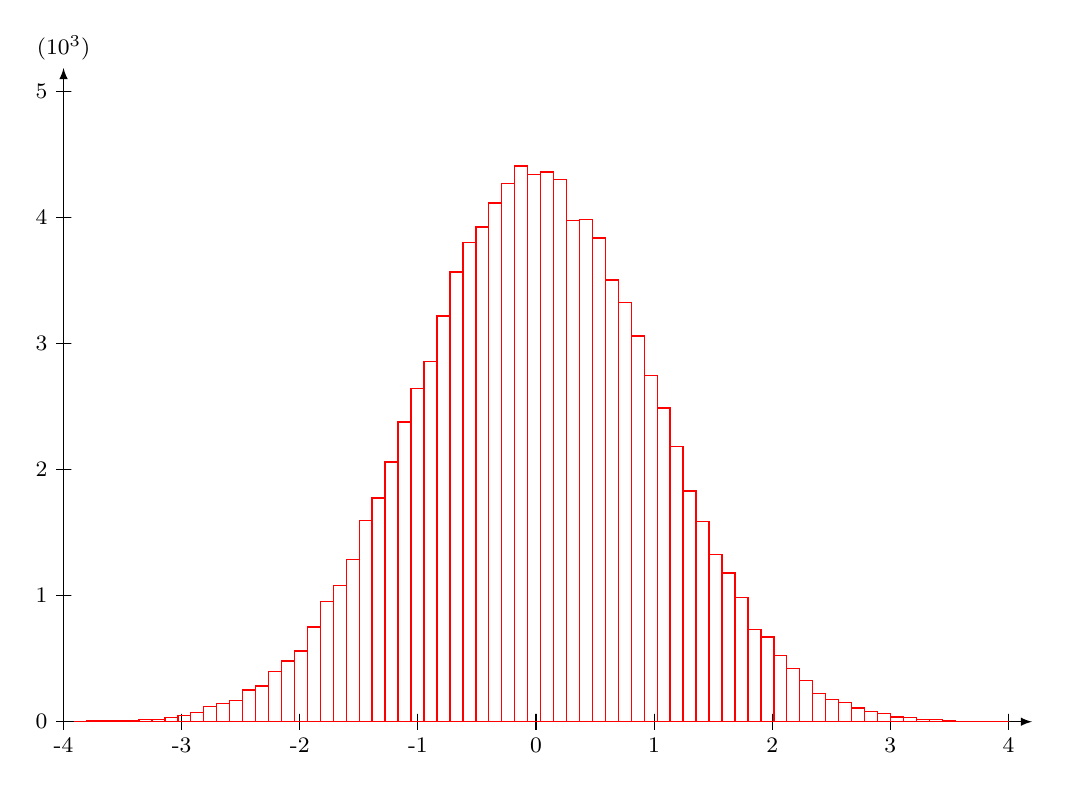
\begin{tikzpicture}[x=0.015cm, y=0.016cm]
\footnotesize
\draw [-latex] ([xshift=-0mm] 0.0,0) -- ([xshift=3mm] 800.0,0) node[right] { };
\draw (0.0,0) -- +(0mm,1mm) -- +(0mm,-1mm) node[below] {-4};
\draw (100.0,0) -- +(0mm,1mm) -- +(0mm,-1mm) node[below] {-3};
\draw (200.0,0) -- +(0mm,1mm) -- +(0mm,-1mm) node[below] {-2};
\draw (300.0,0) -- +(0mm,1mm) -- +(0mm,-1mm) node[below] {-1};
\draw (400.0,0) -- +(0mm,1mm) -- +(0mm,-1mm) node[below] {0};
\draw (500.0,0) -- +(0mm,1mm) -- +(0mm,-1mm) node[below] {1};
\draw (600.0,0) -- +(0mm,1mm) -- +(0mm,-1mm) node[below] {2};
\draw (700.0,0) -- +(0mm,1mm) -- +(0mm,-1mm) node[below] {3};
\draw (800.0,0) -- +(0mm,1mm) -- +(0mm,-1mm) node[below] {4};
\draw [-latex] ([yshift=-0mm] 0,0.0) -- ([yshift=3mm] 0, 500.0) node[above] {  $(10^{3})$};
\draw (0,0.0) -- +(1mm,0mm) -- +(-1mm,0mm) node[left] {0};
\draw (0,100.0) -- +(1mm,0mm) -- +(-1mm,0mm) node[left] {1};
\draw (0,200.0) -- +(1mm,0mm) -- +(-1mm,0mm) node[left] {2};
\draw (0,300.0) -- +(1mm,0mm) -- +(-1mm,0mm) node[left] {3};
\draw (0,400.0) -- +(1mm,0mm) -- +(-1mm,0mm) node[left] {4};
\draw (0,500.0) -- +(1mm,0mm) -- +(-1mm,0mm) node[left] {5};
\draw [line width=0.50pt, color=red] ([xshift=0.0000] 9.0228, 0.0000) rectangle ([xshift=-0.0000] 19.9923, 0.4000); %
\draw [line width=0.50pt, color=red] ([xshift=0.0000] 19.9923, 0.0000) rectangle ([xshift=-0.0000] 30.9618, 0.5000); %
\draw [line width=0.50pt, color=red] ([xshift=0.0000] 30.9618, 0.0000) rectangle ([xshift=-0.0000] 41.9313, 0.6000); %
\draw [line width=0.50pt, color=red] ([xshift=0.0000] 41.9313, 0.0000) rectangle ([xshift=-0.0000] 52.9008, 1.0000); %
\draw [line width=0.50pt, color=red] ([xshift=0.0000] 52.9008, 0.0000) rectangle ([xshift=-0.0000] 63.8703, 1.0000); %
\draw [line width=0.50pt, color=red] ([xshift=0.0000] 63.8703, 0.0000) rectangle ([xshift=-0.0000] 74.8398, 1.9000); %
\draw [line width=0.50pt, color=red] ([xshift=0.0000] 74.8398, 0.0000) rectangle ([xshift=-0.0000] 85.8093, 1.7000); %
\draw [line width=0.50pt, color=red] ([xshift=0.0000] 85.8093, 0.0000) rectangle ([xshift=-0.0000] 96.7788, 3.5000); %
\draw [line width=0.50pt, color=red] ([xshift=0.0000] 96.7788, 0.0000) rectangle ([xshift=-0.0000] 107.7482, 4.9000); %
\draw [line width=0.50pt, color=red] ([xshift=0.0000] 107.7482, 0.0000) rectangle ([xshift=-0.0000] 118.7177, 7.1000); %
\draw [line width=0.50pt, color=red] ([xshift=0.0000] 118.7177, 0.0000) rectangle ([xshift=-0.0000] 129.6872, 12.3000); %
\draw [line width=0.50pt, color=red] ([xshift=0.0000] 129.6872, 0.0000) rectangle ([xshift=-0.0000] 140.6567, 14.7000); %
\draw [line width=0.50pt, color=red] ([xshift=0.0000] 140.6567, 0.0000) rectangle ([xshift=-0.0000] 151.6262, 16.8000); %
\draw [line width=0.50pt, color=red] ([xshift=0.0000] 151.6262, 0.0000) rectangle ([xshift=-0.0000] 162.5957, 25.1000); %
\draw [line width=0.50pt, color=red] ([xshift=0.0000] 162.5957, 0.0000) rectangle ([xshift=-0.0000] 173.5652, 28.4000); %
\draw [line width=0.50pt, color=red] ([xshift=0.0000] 173.5652, 0.0000) rectangle ([xshift=-0.0000] 184.5347, 40.0000); %
\draw [line width=0.50pt, color=red] ([xshift=0.0000] 184.5347, 0.0000) rectangle ([xshift=-0.0000] 195.5042, 48.3000); %
\draw [line width=0.50pt, color=red] ([xshift=0.0000] 195.5042, 0.0000) rectangle ([xshift=-0.0000] 206.4737, 56.2000); %
\draw [line width=0.50pt, color=red] ([xshift=0.0000] 206.4737, 0.0000) rectangle ([xshift=-0.0000] 217.4432, 75.1000); %
\draw [line width=0.50pt, color=red] ([xshift=0.0000] 217.4432, 0.0000) rectangle ([xshift=-0.0000] 228.4127, 95.4000); %
\draw [line width=0.50pt, color=red] ([xshift=0.0000] 228.4127, 0.0000) rectangle ([xshift=-0.0000] 239.3822, 108.2000); %
\draw [line width=0.50pt, color=red] ([xshift=0.0000] 239.3822, 0.0000) rectangle ([xshift=-0.0000] 250.3517, 128.9000); %
\draw [line width=0.50pt, color=red] ([xshift=0.0000] 250.3517, 0.0000) rectangle ([xshift=-0.0000] 261.3212, 159.8000); %
\draw [line width=0.50pt, color=red] ([xshift=0.0000] 261.3212, 0.0000) rectangle ([xshift=-0.0000] 272.2907, 177.4000); %
\draw [line width=0.50pt, color=red] ([xshift=0.0000] 272.2907, 0.0000) rectangle ([xshift=-0.0000] 283.2602, 206.1000); %
\draw [line width=0.50pt, color=red] ([xshift=0.0000] 283.2602, 0.0000) rectangle ([xshift=-0.0000] 294.2297, 237.9000); %
\draw [line width=0.50pt, color=red] ([xshift=0.0000] 294.2297, 0.0000) rectangle ([xshift=-0.0000] 305.1992, 264.5000); %
\draw [line width=0.50pt, color=red] ([xshift=0.0000] 305.1992, 0.0000) rectangle ([xshift=-0.0000] 316.1686, 285.9000); %
\draw [line width=0.50pt, color=red] ([xshift=0.0000] 316.1686, 0.0000) rectangle ([xshift=-0.0000] 327.1381, 321.8000); %
\draw [line width=0.50pt, color=red] ([xshift=0.0000] 327.1381, 0.0000) rectangle ([xshift=-0.0000] 338.1076, 356.8000); %
\draw [line width=0.50pt, color=red] ([xshift=0.0000] 338.1076, 0.0000) rectangle ([xshift=-0.0000] 349.0771, 380.3000); %
\draw [line width=0.50pt, color=red] ([xshift=0.0000] 349.0771, 0.0000) rectangle ([xshift=-0.0000] 360.0466, 392.6000); %
\draw [line width=0.50pt, color=red] ([xshift=0.0000] 360.0466, 0.0000) rectangle ([xshift=-0.0000] 371.0161, 411.6000); %
\draw [line width=0.50pt, color=red] ([xshift=0.0000] 371.0161, 0.0000) rectangle ([xshift=-0.0000] 381.9856, 427.0000); %
\draw [line width=0.50pt, color=red] ([xshift=0.0000] 381.9856, 0.0000) rectangle ([xshift=-0.0000] 392.9551, 440.8000); %
\draw [line width=0.50pt, color=red] ([xshift=0.0000] 392.9551, 0.0000) rectangle ([xshift=-0.0000] 403.9246, 434.2000); %
\draw [line width=0.50pt, color=red] ([xshift=0.0000] 403.9246, 0.0000) rectangle ([xshift=-0.0000] 414.8941, 436.1000); %
\draw [line width=0.50pt, color=red] ([xshift=0.0000] 414.8941, 0.0000) rectangle ([xshift=-0.0000] 425.8636, 430.2000); %
\draw [line width=0.50pt, color=red] ([xshift=0.0000] 425.8636, 0.0000) rectangle ([xshift=-0.0000] 436.8331, 397.7000); %
\draw [line width=0.50pt, color=red] ([xshift=0.0000] 436.8331, 0.0000) rectangle ([xshift=-0.0000] 447.8026, 398.4000); %
\draw [line width=0.50pt, color=red] ([xshift=0.0000] 447.8026, 0.0000) rectangle ([xshift=-0.0000] 458.7721, 383.8000); %
\draw [line width=0.50pt, color=red] ([xshift=0.0000] 458.7721, 0.0000) rectangle ([xshift=-0.0000] 469.7416, 350.4000); %
\draw [line width=0.50pt, color=red] ([xshift=0.0000] 469.7416, 0.0000) rectangle ([xshift=-0.0000] 480.7111, 332.7000); %
\draw [line width=0.50pt, color=red] ([xshift=0.0000] 480.7111, 0.0000) rectangle ([xshift=-0.0000] 491.6806, 306.1000); %
\draw [line width=0.50pt, color=red] ([xshift=0.0000] 491.6806, 0.0000) rectangle ([xshift=-0.0000] 502.6501, 274.7000); %
\draw [line width=0.50pt, color=red] ([xshift=0.0000] 502.6501, 0.0000) rectangle ([xshift=-0.0000] 513.6196, 248.9000); %
\draw [line width=0.50pt, color=red] ([xshift=0.0000] 513.6196, 0.0000) rectangle ([xshift=-0.0000] 524.5891, 218.4000); %
\draw [line width=0.50pt, color=red] ([xshift=0.0000] 524.5891, 0.0000) rectangle ([xshift=-0.0000] 535.5585, 183.2000); %
\draw [line width=0.50pt, color=red] ([xshift=0.0000] 535.5585, 0.0000) rectangle ([xshift=-0.0000] 546.5280, 158.9000); %
\draw [line width=0.50pt, color=red] ([xshift=0.0000] 546.5280, 0.0000) rectangle ([xshift=-0.0000] 557.4975, 132.5000); %
\draw [line width=0.50pt, color=red] ([xshift=0.0000] 557.4975, 0.0000) rectangle ([xshift=-0.0000] 568.4670, 117.9000); %
\draw [line width=0.50pt, color=red] ([xshift=0.0000] 568.4670, 0.0000) rectangle ([xshift=-0.0000] 579.4365, 98.6000); %
\draw [line width=0.50pt, color=red] ([xshift=0.0000] 579.4365, 0.0000) rectangle ([xshift=-0.0000] 590.4060, 73.3000); %
\draw [line width=0.50pt, color=red] ([xshift=0.0000] 590.4060, 0.0000) rectangle ([xshift=-0.0000] 601.3755, 67.3000); %
\draw [line width=0.50pt, color=red] ([xshift=0.0000] 601.3755, 0.0000) rectangle ([xshift=-0.0000] 612.3450, 52.4000); %
\draw [line width=0.50pt, color=red] ([xshift=0.0000] 612.3450, 0.0000) rectangle ([xshift=-0.0000] 623.3145, 42.3000); %
\draw [line width=0.50pt, color=red] ([xshift=0.0000] 623.3145, 0.0000) rectangle ([xshift=-0.0000] 634.2840, 32.7000); %
\draw [line width=0.50pt, color=red] ([xshift=0.0000] 634.2840, 0.0000) rectangle ([xshift=-0.0000] 645.2535, 22.5000); %
\draw [line width=0.50pt, color=red] ([xshift=0.0000] 645.2535, 0.0000) rectangle ([xshift=-0.0000] 656.2230, 17.7000); %
\draw [line width=0.50pt, color=red] ([xshift=0.0000] 656.2230, 0.0000) rectangle ([xshift=-0.0000] 667.1925, 15.2000); %
\draw [line width=0.50pt, color=red] ([xshift=0.0000] 667.1925, 0.0000) rectangle ([xshift=-0.0000] 678.1620, 10.8000); %
\draw [line width=0.50pt, color=red] ([xshift=0.0000] 678.1620, 0.0000) rectangle ([xshift=-0.0000] 689.1315, 8.3000); %
\draw [line width=0.50pt, color=red] ([xshift=0.0000] 689.1315, 0.0000) rectangle ([xshift=-0.0000] 700.1010, 6.4000); %
\draw [line width=0.50pt, color=red] ([xshift=0.0000] 700.1010, 0.0000) rectangle ([xshift=-0.0000] 711.0705, 3.8000); %
\draw [line width=0.50pt, color=red] ([xshift=0.0000] 711.0705, 0.0000) rectangle ([xshift=-0.0000] 722.0400, 3.3000); %
\draw [line width=0.50pt, color=red] ([xshift=0.0000] 722.0400, 0.0000) rectangle ([xshift=-0.0000] 733.0095, 1.8000); %
\draw [line width=0.50pt, color=red] ([xshift=0.0000] 733.0095, 0.0000) rectangle ([xshift=-0.0000] 743.9789, 1.7000); %
\draw [line width=0.50pt, color=red] ([xshift=0.0000] 743.9789, 0.0000) rectangle ([xshift=-0.0000] 754.9484, 1.0000); %
\draw [line width=0.50pt, color=red] ([xshift=0.0000] 754.9484, 0.0000) rectangle ([xshift=-0.0000] 765.9179, 0.3000); %
\draw [line width=0.50pt, color=red] ([xshift=0.0000] 765.9179, 0.0000) rectangle ([xshift=-0.0000] 776.8874, 0.2000); %
\draw [line width=0.50pt, color=red] ([xshift=0.0000] 776.8874, 0.0000) rectangle ([xshift=-0.0000] 787.8569, 0.4000); %
\draw [line width=0.50pt, color=red] ([xshift=0.0000] 787.8569, 0.0000) rectangle ([xshift=-0.0000] 798.8264, 0.4000); %
\draw [line width=0.50pt, color=red] ([xshift=0.0000] 798.8264, 0.0000) rectangle ([xshift=-0.0000] 800.0000, 0.3000); %
\end{tikzpicture}
\end{center}

\caption{A simple histogram for the standard normal density\label{fig:histo1-res}}
\end{figure}

%%%%%%%%%%%%%%%%%%%%%%%%%%%%%%%%%%%%%%%%%%%%%%

The next example, given in Listing~\ref{lst:histochart}, shows how to plot
and customize histograms. First, the two histogram charts \texttt{data1} and
\texttt{data2} are created. Then the data plots are customized: two colors
are selected in the sRGB model from the \texttt{java.awt.Color} package.
40 bins are selected on the interval $[-6, 6]$ for the first histogram.
The number of bins for the second histogram is set automatically.
The range of the plot is set manually with \texttt{bounds}.
 Finally, the two histograms
charts are exported  to file \texttt{HistogramChartTest.tex} in
\LaTeX{} format.  Figure~\ref{fig:histochart-res} displays the resulting chart.


\lstinputlisting[label=lst:histochart,%
caption={Source code creating and customizing histograms.},%
lineskip=-1pt,%
emph={getPoints1,getPoints2,main}
]{exam/HistogramChartTest.java}


\begin{figure}

% PGF/TikZ picture from SSJ 
% XScale = 100.0,  YScale = 0.01,  XShift = 0.0,  YShift = 0.0
% Therefore, thisFileXValue = (originalSeriesXValue+XShift)*XScale
%        and thisFileYValue = (originalSeriesYValue+YShift)*YScale

\begin{center}
\begin{tikzpicture}[x=0.01cm, y=0.02666666666666667cm]
\footnotesize
\draw [latex-latex] ([xshift=-3mm] -600.0,0) -- ([xshift=3mm] 600.0,0) node[right] { };
\draw (0.0,0) -- +(0mm,1mm) -- +(0mm,-1mm) node[below] {0};
\draw (250.0,0) -- +(0mm,1mm) -- +(0mm,-1mm) node[below] {2.5};
\draw (500.0,0) -- +(0mm,1mm) -- +(0mm,-1mm) node[below] {5};
\draw (-250.0,0) -- +(0mm,1mm) -- +(0mm,-1mm) node[below] {-2.5};
\draw (-500.0,0) -- +(0mm,1mm) -- +(0mm,-1mm) node[below] {-5};
\draw [-latex] ([yshift=-0mm] 0,0.0) -- ([yshift=3mm] 0, 300.0) node[above] {  $(10^{4})$};
\draw (0,0.0) -- +(1mm,0mm) -- +(-1mm,0mm) node[above left] {0};
\draw (0,125.0) -- +(1mm,0mm) -- +(-1mm,0mm) node[left] {1.25};
\draw (0,250.0) -- +(1mm,0mm) -- +(-1mm,0mm) node[left] {2.5};
\draw [line width=0.50pt, color=green] ([xshift=0.0000] 0.0025, 0.0000) rectangle ([xshift=-0.0000] 34.9737, 294.9100); %
\draw [line width=0.50pt, color=green] ([xshift=0.0000] 34.9737, 0.0000) rectangle ([xshift=-0.0000] 69.9450, 207.8600); %
\draw [line width=0.50pt, color=green] ([xshift=0.0000] 69.9450, 0.0000) rectangle ([xshift=-0.0000] 104.9162, 147.4900); %
\draw [line width=0.50pt, color=green] ([xshift=0.0000] 104.9162, 0.0000) rectangle ([xshift=-0.0000] 139.8875, 103.3800); %
\draw [line width=0.50pt, color=green] ([xshift=0.0000] 139.8875, 0.0000) rectangle ([xshift=-0.0000] 174.8587, 73.0000); %
\draw [line width=0.50pt, color=green] ([xshift=0.0000] 174.8587, 0.0000) rectangle ([xshift=-0.0000] 209.8300, 50.3900); %
\draw [line width=0.50pt, color=green] ([xshift=0.0000] 209.8300, 0.0000) rectangle ([xshift=-0.0000] 244.8012, 37.1400); %
\draw [line width=0.50pt, color=green] ([xshift=0.0000] 244.8012, 0.0000) rectangle ([xshift=-0.0000] 279.7725, 25.8700); %
\draw [line width=0.50pt, color=green] ([xshift=0.0000] 279.7725, 0.0000) rectangle ([xshift=-0.0000] 314.7437, 17.5400); %
\draw [line width=0.50pt, color=green] ([xshift=0.0000] 314.7437, 0.0000) rectangle ([xshift=-0.0000] 349.7150, 12.5400); %
\draw [line width=0.50pt, color=green] ([xshift=0.0000] 349.7150, 0.0000) rectangle ([xshift=-0.0000] 384.6862, 8.9700); %
\draw [line width=0.50pt, color=green] ([xshift=0.0000] 384.6862, 0.0000) rectangle ([xshift=-0.0000] 419.6575, 6.3400); %
\draw [line width=0.50pt, color=green] ([xshift=0.0000] 419.6575, 0.0000) rectangle ([xshift=-0.0000] 454.6287, 4.1600); %
\draw [line width=0.50pt, color=green] ([xshift=0.0000] 454.6287, 0.0000) rectangle ([xshift=-0.0000] 489.6000, 3.0000); %
\draw [line width=0.50pt, color=green] ([xshift=0.0000] 489.6000, 0.0000) rectangle ([xshift=-0.0000] 524.5712, 2.3400); %
\draw [line width=0.50pt, color=green] ([xshift=0.0000] 524.5712, 0.0000) rectangle ([xshift=-0.0000] 559.5425, 1.3100); %
\draw [line width=0.50pt, color=green] ([xshift=0.0000] 559.5425, 0.0000) rectangle ([xshift=-0.0000] 594.5137, 1.2300); %
\draw [line width=0.50pt, color=green] ([xshift=0.0000] 594.5137, 0.0000) rectangle ([xshift=-0.0000] 600.0000, 0.7400); %
\draw [line width=0.50pt, color=red] ([xshift=0.0000] -600.0000, 0.0000) rectangle ([xshift=-0.0000] -570.0000, 0.8900); %
\draw [line width=0.50pt, color=red] ([xshift=0.0000] -570.0000, 0.0000) rectangle ([xshift=-0.0000] -540.0000, 1.1600); %
\draw [line width=0.50pt, color=red] ([xshift=0.0000] -540.0000, 0.0000) rectangle ([xshift=-0.0000] -510.0000, 2.0500); %
\draw [line width=0.50pt, color=red] ([xshift=0.0000] -510.0000, 0.0000) rectangle ([xshift=-0.0000] -480.0000, 2.7500); %
\draw [line width=0.50pt, color=red] ([xshift=0.0000] -480.0000, 0.0000) rectangle ([xshift=-0.0000] -450.0000, 4.1400); %
\draw [line width=0.50pt, color=red] ([xshift=0.0000] -450.0000, 0.0000) rectangle ([xshift=-0.0000] -420.0000, 5.5800); %
\draw [line width=0.50pt, color=red] ([xshift=0.0000] -420.0000, 0.0000) rectangle ([xshift=-0.0000] -390.0000, 7.5300); %
\draw [line width=0.50pt, color=red] ([xshift=0.0000] -390.0000, 0.0000) rectangle ([xshift=-0.0000] -360.0000, 10.2600); %
\draw [line width=0.50pt, color=red] ([xshift=0.0000] -360.0000, 0.0000) rectangle ([xshift=-0.0000] -330.0000, 13.0900); %
\draw [line width=0.50pt, color=red] ([xshift=0.0000] -330.0000, 0.0000) rectangle ([xshift=-0.0000] -300.0000, 17.1400); %
\draw [line width=0.50pt, color=red] ([xshift=0.0000] -300.0000, 0.0000) rectangle ([xshift=-0.0000] -270.0000, 22.9000); %
\draw [line width=0.50pt, color=red] ([xshift=0.0000] -270.0000, 0.0000) rectangle ([xshift=-0.0000] -240.0000, 26.2900); %
\draw [line width=0.50pt, color=red] ([xshift=0.0000] -240.0000, 0.0000) rectangle ([xshift=-0.0000] -210.0000, 32.1400); %
\draw [line width=0.50pt, color=red] ([xshift=0.0000] -210.0000, 0.0000) rectangle ([xshift=-0.0000] -180.0000, 37.4900); %
\draw [line width=0.50pt, color=red] ([xshift=0.0000] -180.0000, 0.0000) rectangle ([xshift=-0.0000] -150.0000, 42.8600); %
\draw [line width=0.50pt, color=red] ([xshift=0.0000] -150.0000, 0.0000) rectangle ([xshift=-0.0000] -120.0000, 46.8800); %
\draw [line width=0.50pt, color=red] ([xshift=0.0000] -120.0000, 0.0000) rectangle ([xshift=-0.0000] -90.0000, 51.6000); %
\draw [line width=0.50pt, color=red] ([xshift=0.0000] -90.0000, 0.0000) rectangle ([xshift=-0.0000] -60.0000, 55.1300); %
\draw [line width=0.50pt, color=red] ([xshift=0.0000] -60.0000, 0.0000) rectangle ([xshift=-0.0000] -30.0000, 57.7000); %
\draw [line width=0.50pt, color=red] ([xshift=0.0000] -30.0000, 0.0000) rectangle ([xshift=-0.0000] 0.0000, 60.5300); %
\draw [line width=0.50pt, color=red] ([xshift=0.0000] 0.0000, 0.0000) rectangle ([xshift=-0.0000] 30.0000, 59.7400); %
\draw [line width=0.50pt, color=red] ([xshift=0.0000] 30.0000, 0.0000) rectangle ([xshift=-0.0000] 60.0000, 59.1500); %
\draw [line width=0.50pt, color=red] ([xshift=0.0000] 60.0000, 0.0000) rectangle ([xshift=-0.0000] 90.0000, 56.5200); %
\draw [line width=0.50pt, color=red] ([xshift=0.0000] 90.0000, 0.0000) rectangle ([xshift=-0.0000] 120.0000, 52.6300); %
\draw [line width=0.50pt, color=red] ([xshift=0.0000] 120.0000, 0.0000) rectangle ([xshift=-0.0000] 150.0000, 47.8100); %
\draw [line width=0.50pt, color=red] ([xshift=0.0000] 150.0000, 0.0000) rectangle ([xshift=-0.0000] 180.0000, 43.1000); %
\draw [line width=0.50pt, color=red] ([xshift=0.0000] 180.0000, 0.0000) rectangle ([xshift=-0.0000] 210.0000, 36.9200); %
\draw [line width=0.50pt, color=red] ([xshift=0.0000] 210.0000, 0.0000) rectangle ([xshift=-0.0000] 240.0000, 30.9900); %
\draw [line width=0.50pt, color=red] ([xshift=0.0000] 240.0000, 0.0000) rectangle ([xshift=-0.0000] 270.0000, 26.6600); %
\draw [line width=0.50pt, color=red] ([xshift=0.0000] 270.0000, 0.0000) rectangle ([xshift=-0.0000] 300.0000, 21.0800); %
\draw [line width=0.50pt, color=red] ([xshift=0.0000] 300.0000, 0.0000) rectangle ([xshift=-0.0000] 330.0000, 16.9000); %
\draw [line width=0.50pt, color=red] ([xshift=0.0000] 330.0000, 0.0000) rectangle ([xshift=-0.0000] 360.0000, 13.8300); %
\draw [line width=0.50pt, color=red] ([xshift=0.0000] 360.0000, 0.0000) rectangle ([xshift=-0.0000] 390.0000, 9.9100); %
\draw [line width=0.50pt, color=red] ([xshift=0.0000] 390.0000, 0.0000) rectangle ([xshift=-0.0000] 420.0000, 7.3800); %
\draw [line width=0.50pt, color=red] ([xshift=0.0000] 420.0000, 0.0000) rectangle ([xshift=-0.0000] 450.0000, 5.4600); %
\draw [line width=0.50pt, color=red] ([xshift=0.0000] 450.0000, 0.0000) rectangle ([xshift=-0.0000] 480.0000, 4.1800); %
\draw [line width=0.50pt, color=red] ([xshift=0.0000] 480.0000, 0.0000) rectangle ([xshift=-0.0000] 510.0000, 2.6900); %
\draw [line width=0.50pt, color=red] ([xshift=0.0000] 510.0000, 0.0000) rectangle ([xshift=-0.0000] 540.0000, 2.0300); %
\draw [line width=0.50pt, color=red] ([xshift=0.0000] 540.0000, 0.0000) rectangle ([xshift=-0.0000] 570.0000, 1.3500); %
\draw [line width=0.50pt, color=red] ([xshift=0.0000] 570.0000, 0.0000) rectangle ([xshift=-0.0000] 600.0000, 0.9400); %
\end{tikzpicture}
\end{center}

\caption{A customized histogram chart\label{fig:histochart-res}}
\end{figure}

%%%%%%%%%%%%%%%%%%%%%%%%%%%%%%%%%%%%%%%%%%%%%%


The next example, given in Listing~\ref{lst:boxplot}, shows how to create
a box-and-whisker plot. First, two series of 1000 points
are obtained from a lognormal distribution and from a Poisson distribution
with $\lambda=5$. These are passed to a \texttt{BoxChart} object, which
creates the boxplot, which can be viewed on screen by executing
the program. We find that the boxplot for the Poisson data (the box on the right
of the chart) has median = 5
(the line inside the box), a mean = 5.009 (the center of the black circle)
the first and the third quartiles at 3 and 6, while the lower and upper
whiskers are at 0 and 10. Finally, there are outliers at 11 and 12 (the hollow
circles) and extreme outliers (the triangle) at 13, outside the chart.
We see that the Poisson data is skewed towards higher values.
A similar description applies to the lognormal data (the box on the left
of the chart), which is strongly skewed towards smaller values.

\lstinputlisting[label=lst:boxplot,%
caption={Source code creating a box-and-whisker plot.},%
lineskip=-1pt,%
emph={main}
]{exam/BoxTest.java}

\vspace{1cm}

\begin{figure}
\begin{center}
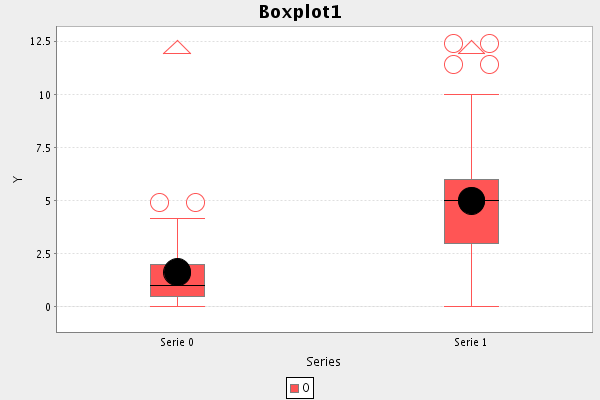
\includegraphics[scale=0.5]{exam/BoxTest.png}
\caption{A box-plot\label{fig:boxchart-res}}
\end{center}
\end{figure}
%%%%%%%%%%%%%%%%%%%%%%%%%%%%%%%%%%%%%%%%%%%%%%

\end{latexonly}
